%!TEX root =  proposal.tex

\section{Computational biology applications}


\subsection{Taxonomic classification of metagenomic data}

{\bf Problem definition.}
The microbes that live in an environment can be identified by their combined genomic material, also called the metagenome.
The study of metagenomes provides an opportunity to closely examine complex biological interactions, such as phage-host and metabolic dynamics~\cite{national2007new}.
Metagenomic datasets contain sequencing reads from multiple species that are present in the biological environment.
%
Taxonomic classification~\cite{wood2014kraken} helps to identify the microbial taxon or taxa present in large-scale  metagenomic datasets coming from complex biological and environmental samples. Assigning taxonomic labels to sequencing reads is an important part of many computational genomics pipelines for metagenomics projects.

\noindent
{\bf Importance.}
Taxonomic classification of reads is a critical first computational step in any metagenomic analysis pipeline.
For example, read classification is critical for \emph{de novo} metagenomics assembly, which attempts to reconstruct the DNA sequence of each organism present in the metagenomic sample without using a reference database before performing the actual assembly step~\cite{venter2004environmental,brady2009phymm,brady2011phymmbl,rosen2008metagenome,segata2012metagenomic}.

\noindent
{\bf Challenges.}
The task of read classification is far from straightforward. 
A metagenomic sample can contain thousands of genomes with varying level of similarity and often occurring at vastly different abundances. Furthermore, due to high-throughput sequencing metagenomic datasets contains millions of sequencing reads making traditional, string-matching-based tools like BLAST infeasible to perform classification. Metagenomic datasets today easily range from hundreds of GBs to TBs. For example, WA dataset contains a collection of marine microbial communities from the Western Arctic Ocean and consists of 822 GB of 2.5 billion reads in 12 samples~\cite{hofmeyr2020terabase}.

\noindent
{\bf State of the art.}
Taxonomic classification tools~\cite{ames2013scalable, kim2016centrifuge, menzel2016fast, wood2014kraken, wood2019improved, dilthey2019strain,liu2018novel} use a supervised approach to assign taxonomic labels to reads.
These tools build a database of known genomes and their taxonomic labels from the NCBI database.
The database is typically an index that maps smaller subsequences (\kmers) to the list of taxa corresponding to the genomes in which the subsequences occur.
During the classification phase, the input reads are decomposed into \kmers and queried in the index to determine the most appropriate taxon.

\noindent
{\bf Gaps and requirements.}
The sheer size of sequenced microbial genetic sequences presents a considerable computational challenge.
Building the database of known genomes is often quite memory intensive.
The most popular reference database are RefSeq complete genomes (RefSeq CG) for microbial species as well as the BLAST nt and nr databases for high-quality nucleotide and protein sequences, respectively, with $\approx50$ and $\approx200$ millon sequences.
Kraken's~\cite{wood2014kraken} memory requirements can easily exceed 100GB~\cite{simon2019benchmarking}, especially when the reference data includes large eukaryotic genomes~\cite{meiser2017sequencing, knutson2017porcine}.
%
The universe of microbial sequences is large and diverse. The vast search space often results in false positives as sequences can be matched against multiple taxa. Also, a large number of undiscovered microbial species can result in false negatives as these species are not present in the database.

Existing taxonomic classification tools are memory intensive to build the database of known genomes and often require more memory than available on single-node machines. Furthermore, classification operation is computationally intensive and makes it infeasible to scale to terabyte-scale metagenomic datasets.
%
Furthermore, existing reference database indexes give up updatability to save space. However, the ability to add new assembled genomes to an existing database is a critical feature to avoid rebuilding the databases. 


\begin{rproblem}[\textbf{Metagenomic classification at terabyte scale}]
Build a software tool to perform reference-based taxnomic classification of metagenomic reads for terabyte-scale metagenomic datasets. Furthermore, the software tool should support adding new assembled genomes to the database and updating the labels of existing ones without rebuilding the database.
\label{rprob:peppermint1}
\end{rproblem}

% \mfc{there is no discussion of what we are actually going to do.  what hardware?  what tests?  how will we know that we succeeded?  How much of an improvement do we need in order to succeed?  What it will it mean to our target application community if we succeed?}


\subsection{Large-scale raw sequence search}

{\bf Problem statement.} Raw sequence search involves  identifying all sequencing samples in a database of raw sequencing data such as SRA~\cite{kodama2012sequence} that contain a given query sequence. A query is an arbitrary sequence, such as a transcript. Raw sequencing datasets contain a ton of biological diversity information that can be used to answer biological questions that single sequencing sample do not have the power to address.

\noindent
{\bf Importance.}
The vast majority of publicly available sequencing data (e.g., the data deposited in the Sequence Read Archive [SRA]~\cite{kodama2012sequence}) exist in the form of raw, unassembled sequencing reads. The raw sequencing data contains a lot of biological diversity information which is lost during the assembly process. Furthermore, only a small fraction of all the raw sequencing data is assembled, making the raw sequencing data even more important to answer complex biological-diversity related questions. 

\noindent
{\bf Challenges.}
There have been multiple tools such as BLAST~\cite{altschul1990basic} and its variants that are designed to issue \mfc{but not perform?} sequence level searches over publicly available databases of assembled genomes and known proteins. Much subsequent work has focused on how to extend tools such as BLAST to be faster, more sensitive, or both~\cite{XXX}. \mfc{This previous sentence is a jolt. what does that have to do with raw sequence data?}  However, the strategies applied by such tools focus on the case where queries are issued over a database of reference sequences which is much smaller in size compared to the SRA. \mfc{again, what does this have to do with raw sequence data?}
%
There are a number of reasons that typical reference-database-based search techniques cannot easily be applied in the context of searching raw, unassembled sequences. One major reason is that most current techniques do not scale well as the amount of data grows to the size of the SRA (which today is $\approx4$ petabases of sequence information). A second reason is that searching unassembled sequences means that relatively long queries (e.g., genes) are unlikely to be present in their entirety as an approximate substring of the input.
As such, these data have mostly been rendered impervious to sequence-level search, which substantially reduces the utility of such publicly available data.


\noindent
{\bf State of the art.}
Recently, new computational schemes have been proposed
that hold the potential to allow searching raw SARs while overcoming these challenges. Solomon and Kingsford~\cite{solomon2016fast} introduced the sequence bloom tree (SBT) data structure and an associated algorithm that enables an efficient type of search over thousands of sequencing experiments. Specifically, they re-phrase the query in terms of k-mer set membership in a way that is robust to the fact that the target sequences have not been assembled. The resulting problem is coined as the experiment discovery problem, where the goal is to return all experiments that contain at least some user-defined q fraction of the k-mers present in the query string.
%
Subsequently, Mantis~\cite{PandeyABFJP18Cell} was developed by PI Pandey and PI Bender that showed how solve the experiment discovery problem using an inverted-index approach by mapping \kmers to the list of experiments they appear in. Mantis uses the counting quotient filter~\cite{PandeyBJP17} as in exact map to map \kmers. They further continued this effort in collaboration with Prof. Patro UMD to scale Mantis~\cite{AlmodaresiPFJP19,AlmodaresiPFJP20} to storage devices.


\noindent
{\bf Gaps and requirement.}

\prashant{Fill in...}

\begin{rproblem}[\textbf{Build a raw sequence search index over all of SRA}]
Build a \kmer index over all the raw experiments present in SRA~\cite{kodama2012sequence} and enable sequence-level searches in real-time. Furthermore, host the index publicly to make it available for researchers around the world. Researchers can quickly ask biological questions and get answers. For example: what if researchers wants to determine: if a new putative disease-related transcript appeared in other samples, if a new fusion event is
common among samples with a given subtype, which samples contain a new unexpected bacterial contaminant. 
\label{rprob:peppermint2}
\end{rproblem}

\subsection{Pangenomics}

{\bf Problem definition.}
Pangenomics~\cite{garrison2018variation} involves storing the genome of a species as a sequence graph consisting of genomes of multiple individuals instead of a single linear reference. A primary goal of pangenomic variation analysis is to avoid biases that arise when treating a single genome as the reference when identifying or comparing variants across samples in a population.

\noindent
{\bf Importance.}
Much of the field of genomics revolves around the existence of reference genomes, which are roadmaps for a ‘typical’ individual of each species. The creation of each reference was, and still remains, a major focus of the genomics community, with 13 years and US\$2.7 billion having been spent on the creation of the human reference genome alone. The ability to compare a newly sequenced individual with a reference and find differences has enabled myriad discoveries and innovations, and in human genomics this ability has formed the basis of thousands of studies seeking the genetic origins of disease. However, as the number and scope of sequencing experiments have grown dramatically, scientists have begun to realize the many limitations that a single reference genome imposes upon the community. To better capture the variation missed by using one reference, we can create and utilize a ‘pan-genome’, a collection of all the DNA sequences that occur in a species.

\noindent
{\bf Challenges.}
Cataloguing the DNA from all individuals in a species is a daunting task. The first pan-genomes were developed for small, easy-to-sequence bacteria, but, even in that context, pan-genomes provided novel scientific insights. The consideration of genetic diversity within bacterial species has contributed to our understanding of underlying differences in pathogenicity, virulence and drug resistance and can even help predict how pathogenic a new strain will be.

Pan-genome studies of plants and animals remained elusive at first, due to the large genome sizes and vast amounts of intergenic sequence in these species. However, in recent years, thanks to dramatic improvements in the efficiency of sequencing technology, the scientific community has been able to sequence dozens, hundreds or even thousands of individuals of a single plant or animal species~\cite{XXX}. Additionally, new long-read sequencing technologies now allow us to better assemble repetitive regions of large genomes, including centromeric regions, that are difficult to characterize with short reads~\cite{XXX}.

Human sequencing, too, has accelerated. Over the past few years, a flurry of publications have described large collections of newly sequenced human genomes, including population-specific cohorts from Iceland~\cite{XXX}, Denmark~\cite{XXX}, Sweden~\cite{XXX}, Papua New Guinea~\cite{XXX}, Mongolia~\cite{XXX} and Africa~\cite{XXX}, as well as large-scale surveys of the entire world~\cite{XXX}.

\noindent
{\bf State of the art.}
Pangenomic studies are performed by storing the genomes of multiple individuals in a genome graph (also known as the sequence graph or variation graph). A genome graph is a directed, acyclic graph (DAG) $G = (N, E, P)$ that embeds a set of DNA sequences. It comprises a set of nodes $N$, a set of direct edges $E$, and a set of paths $P$. For DNA sequences, we use the alphabet \{A, C, G, T, N\}\@. Each $n_i \in N$ represents a sequence $seq(n_i)$. Edges in the graph connect nodes that are followed on a path. Nodes on a path are assigned positions based on the coordinate systems of sequences they represent.

Efficiently indexing and storing a genome graph is a computationally and memory/space intensive process due to the presence of thousands of coordinate systems corresponding to the individuals. Existing applications that index genome graphs~\cite{pandey2021variantstore,garrison2018variation} are designed to use compressed string indexes and off-the-shelf graph indexes. However, these indexes do not scale to pangenomic datasets available today due the limitations to the memory-intensive characteristics of these data structures. Furthermore, these indexes are not designed to efficiently support adding new genomes to an existing index. They to rebuild the whole index in order to add a new sample.

\noindent
{\bf Gaps and requirement.}
Current pangenomic indexes do not scale to population-scale variation datasets such as 100,000 Genomes project~\cite{1002021100}. Furthermore, they do not support adding new genomes to an existing index. In order to add a new genomic sample to the pangenomic index required rebuilding the complete index.

\begin{rproblem}[\textbf{Building a pangenomic index at population-scale and performing sequence-to-graph mapping}]
 We want to build a pangenomic index that can perform fast variation queries, sequence-to-graph mapping, support updates, and scale to population-scale datasets.
\label{rprob:peppermint3}
\end{rproblem}

\subsection{\kmer analysis for metagenome assembly}
\prashant{Annotate figures to show where's the problem in terms of scale...}


% \begin{figure}
\begin{wrapfigure}{R}{0.7\textwidth}
    \centering
    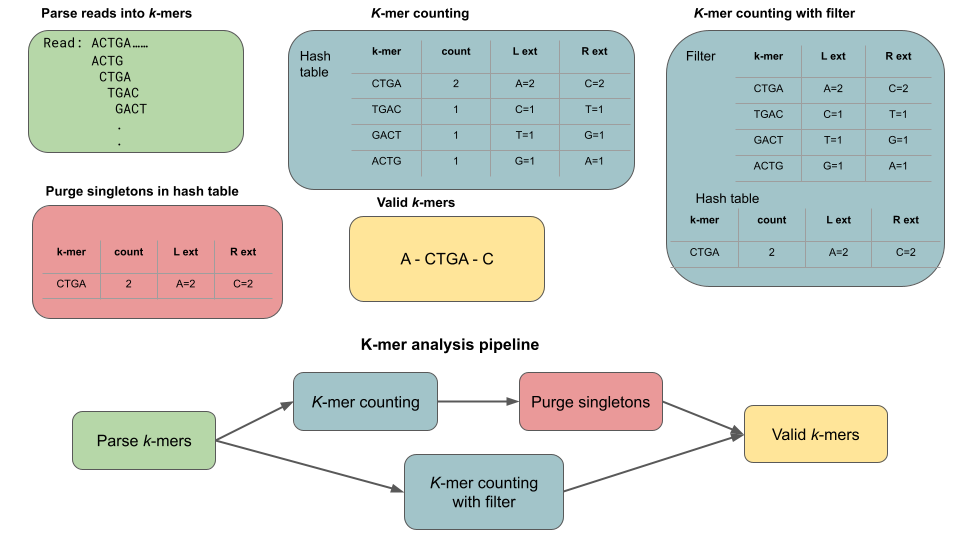
\includegraphics[width=0.9\linewidth]{images/mhm-pipeline.png}
    \caption{The \textit{k}-mer analysis pipeline in MetaHipMer. A filter can help weed out singleton $k$-mers from being inserted into the hash table.}
    \vspace{-0.5em}
    \label{fig:mhm-kmer}
\end{wrapfigure}
% \end{figure}

Metagenome assembly involves reconstructing long contiguous sequences ({\it contigs}) of genetic material from short input {\it reads}. These reads are strings of bases (the DNA alphabet A, C, G, T) of length 150 to 250 that are produced by gene sequencing machines.  For metagenomes, these reads are extracted from environmental samples (e.g., gut bacteria, or a soil sample) that contain the genes of potentially thousands of microbes, existing at varying abundances.  The reads are error prone (typically about 0.24\% error per base) and sequencing is done multiple times to ensure every region of genetic material is covered with some error free sequences.

In the approach used by MetaHipMer~\cite{GeorganasEHG18,HofmeyrEGC20}, the reads are first divided into overlapping substrings of fixed length {\it k}, called {\it $k$-mers}, which are then used to form a de Bruijn graph~\cite{CompeauPeTe11}. In a de Bruijn graph, the vertices are $k$-mers and edges connect any two $k$-mers that have an overlap of $k-1$ bases. These vertices are stored in a hash table that is distributed across all the compute processes.  The size of the hash table is dependent on the number of unique $k$-mers.  Traversal of the de Bruijn graph enables the construction of the contigs (longer sequences).  This approach is more efficient than an all-to-all alignment of the reads, which would be prohibitive for the size of typical metagenome datasets (up to billions of reads).

Forward and backward extensions of the $k$-mer and the counts of those extensions are also maintained in the hash table along with the $k$-mer. Information regarding the extensions and their counts is critical to identifying correct paths in the de Bruijn graph and requires 28 to 52 bytes (depending on $k$) to store each $k$-mer.

To ensure accurate contigs, the $k$-mers that occur only once (singletons) are
treated as errors and dropped. In a typical set of metagenome reads, 70--80\%
of unique $k$-mers are singletons, but they still need to be stored and counted
in the distributed hash table. In the default MetaHipMer implementation, storing the unique $k$-mers is the most memory intensive part of the computation and can be roughly an order of magnitude larger than the input data.  The space required to store the $k$-mers can be much larger than the size of the original raw dataset (up to $10\times$ larger) as $k$-mers contain a lot of redundant information due to their overlaps.



The distributed hash table in MetaHipMer is implemented as a collection of local hash tables, one per process, with communication happening via UPC++ remote procedure calls (RPCs). In the hash table insertion phase, the $k$-mers are aggregated, dispatched over the network, and inserted in bulk into the local hash tables, which are running on GPUs. Using GPUs boosts performance, but further constrains memory (e.g. the Summit supercomputer~\cite{VazhkudaiDBG18} has an aggregate of 96~GB GPU memory and 512~GB CPU memory per node).

MetaHipMer runs on distributed systems with multiple nodes, and each node could have multiple GPUs, e.g. Summit has 6 GPUs per node. To utilize all the GPUs on a node, MetaHipMer maps the UPC++ processes to the GPUs in a round robin fashion, so multiple processes will share each GPU using the NVIDIA Multi-Process Service (MPS)\@. On a Summit node there will be 42 processes (one per core) and hence there will be 7 processes per GPU\@. Using the MPS has the benefits of simplicity, because there is no inter-GPU communication required, and it improves performance by increasing the utilization of the GPUs.


\Cref{fig:mhm-kmer} shows different parts of the $k$-mer analysis phase in
MetaHipMer. In the standard pipeline, all $k$-mers are counted in the hash table and then a separate phase is required to purge all the singleton $k$-mers.

\paragraph{\Kmer distribution}

\begin{wraptable}{r}{4.5in}
\centering
%\resizebox{\columnwidth}{!}{%
    \begin{tabular}{c | c | c | c | c | c}
    \toprule
    \textbf{Dataset} & \multicolumn{5}{c}{\textbf{Percentage singleton $k$-mers}} \\
    \midrule
    & $K=21$ & $k=33$ & $k=55$ & $k=77$ & $k=99$ \\
    \midrule
    WA &  66 & 73 & 76 & 78 & 78  \\
    Rhizo &  67 & 75 & 80 & 83 & 85  \\
    Tymeflies & 63 & 62 & 67 & 69 & 71 \\
    \bottomrule
    \end{tabular}
 %   }
    \caption{Distribution of singleton $k$-mers in metagenomic data for values of $k$.}
    \label{tab:kmer-dist}
\end{wraptable}

\Cref{tab:kmer-dist} shows the distribution of singleton \kmers in three
different metagenomic datasets. Singleton \kmers form a majority fraction of
the total number of distinct \kmers. The distribution often depends on the
sequencing depth and the size of $k$. The larger value $k$ results in larger
fraction of singleton \kmers. This is due to the higher probability of seeing
an erroneous base in the \kmer given the higher value of $k$. The erroneous
bases result in singleton \kmers.

Weeding out singleton \kmers before inserting them in the hash table to count
is critical in any \kmer analysis phase to reduce the memory usage of the
counting phase. These singleton $k$-mers can also be pruned from the hash table
after the counting phase. However, that results in the high peak memory usage
and much slower running time.

Using a space-efficient filter to weed out singleton \kmers helps to reduce
the memory pressure on the counting hash table thereby reducing the peak memory
usage and increased run time. See~\cref{fig:mhm-kmer}.


\noindent
{Challenges.}
So far MetaHipMer is limited by the peak RAM usage in high-performance computing (HPC) environments.

\begin{rproblem}[\textbf{Scale MetaHipMer to petabyte-scale metagenomic datasets on supercomputers}]
Accelerate \kmer analysis phase in MetaHipMer using GPUs and reduce the peak RAM usage to support assembly of petabyte-scale metagenomic datasets from complex biological environments.
\label{rprob:peppermint4}
\end{rproblem}

